\documentclass{standalone}
% 公式
\usepackage{amsmath}
% 公式符号加粗
\usepackage{bm}
% TikZ 图形
\usepackage{tikz}
% 插入三维图形
\usepackage{pgfplots}
\pgfplotsset{width=7cm,compat=1.18}

\begin{document}

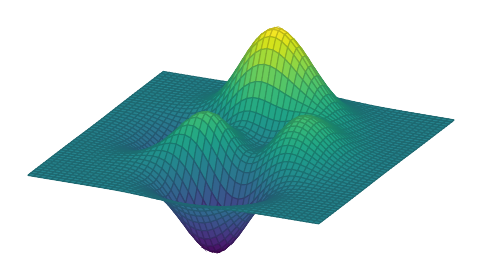
\begin{tikzpicture}
\begin{axis}[
    hide axis,
    colormap/viridis,
]
\addplot3[
    surf,
    samples=50,
    domain=-3:3,
]
{3*(1-x)^2*exp(-x^2 - (y+1)^2) - 10*(x/5 - x^3 -y^5)*exp(-x^2 -y^2) - 1/3*exp(-(x+1)^2 -y^2};
\end{axis}
\end{tikzpicture}

\end{document}
